\chapter{Scraper Design and Implementation}\label{C:us}

In this section I discuss the design and implementation of the web scraping components of the project. I highlight important decisions made during the course of the project, as well as steps taken to implement the system based on requirements detailed in chapter four.

%\section{A Prototyping Approach}

%Talk about how the design was constructed.

%My approach to prototyping and the problems this revealed.

%The overall design of my scrapers was largely developed through a prototyping approach early in the project. I performed research and web-scraping frameworks and technologies to decide which would best suit the requirements defined in chapter 4. The prototyping strategy also allowed me to investigate the feasiblity of scraping from different sites.

%By developing prototypes for Facebook and Twitter early in the project I was better able to 

\section{Architecture}

Through the development of these basic prototypes, construction of more formal architectures was possible. I consider two architectures, when designing the web-scraper components. A database-storage approach was considered, and the more straightforward text/XML storage architecture was also considered and ultimately selected. 

\subsection{Database Storage Architecture}

\begin{figure}[h!]
 \centering
 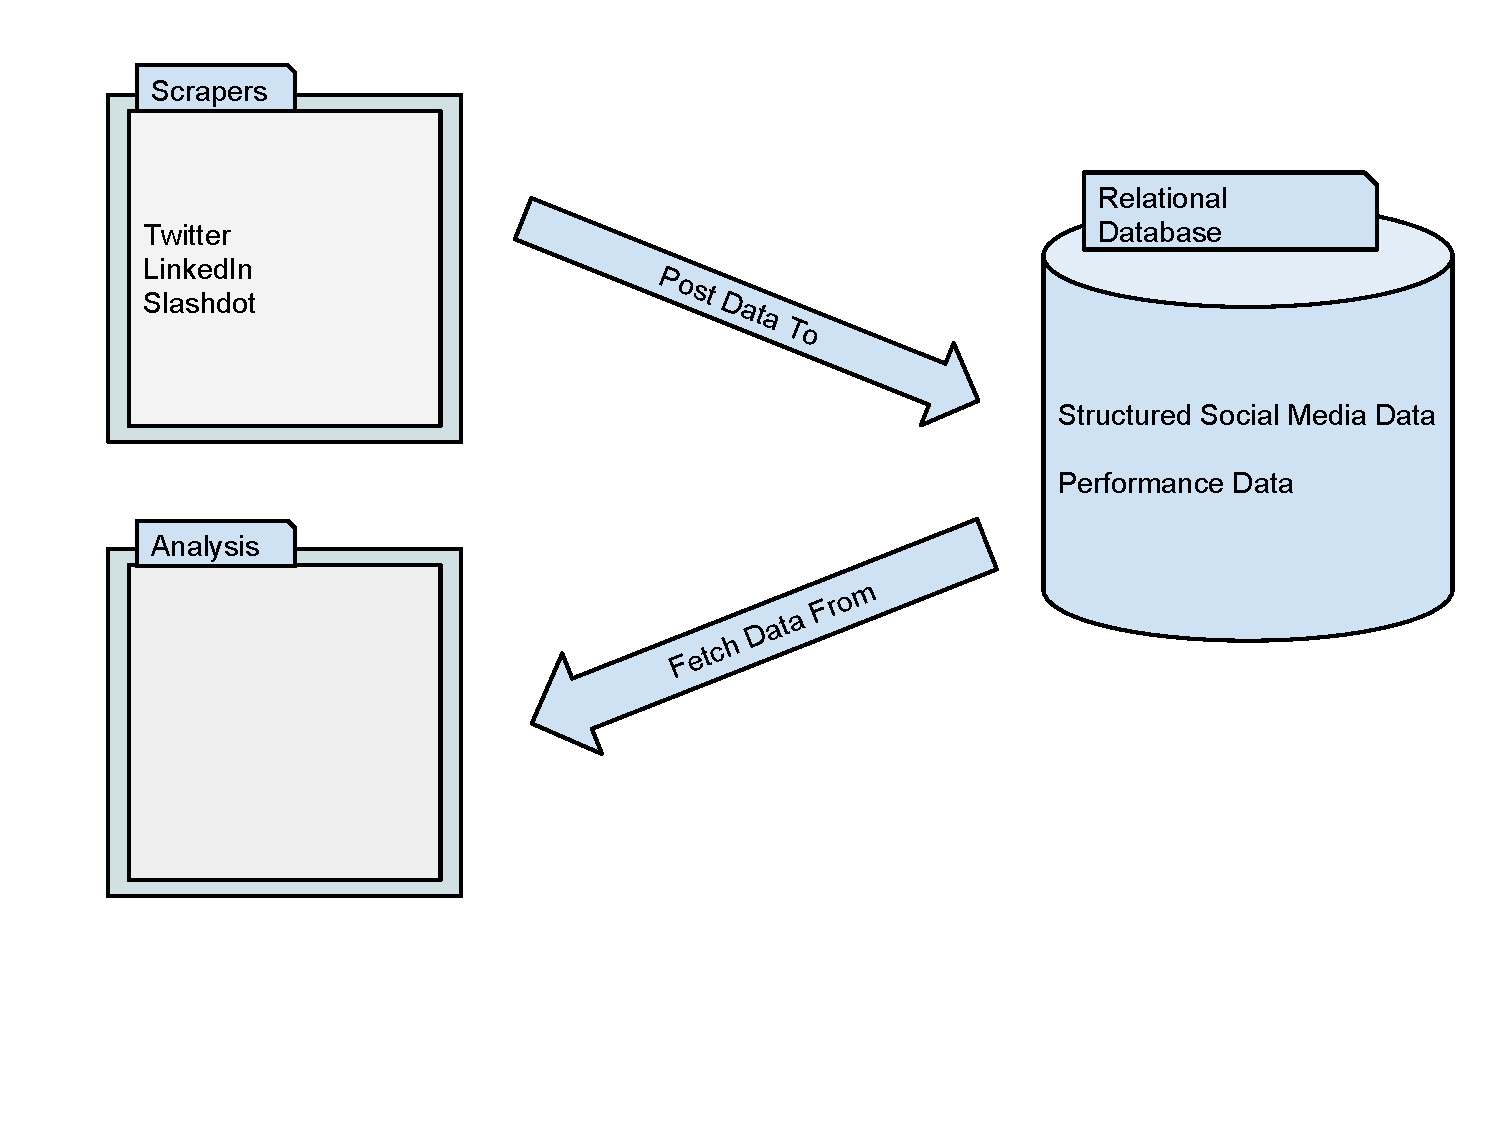
\includegraphics[width=0.7\textwidth]{Images/Database_Architecture.pdf}
 \caption{Proposed Architecture for Database Storage Solution}
\end{figure}

A possible approach to meeting the goals of the project was to store fetched data in a relational database. In this design, the scrapers would gather data over an extended period of time, writing retrieved data into a database. Analysis components would then fetch data from the database storage as necessary, saving results in seperate tables within the same database.

This approach provides benefits in terms of long-term extensibility of the project. All of the advantages that come with database storage would have been present in this solution - fetching of specific profiles for example would have been much more practical through a database query. 

The drawbacks to this approach are to do with the deemed over-engineered nature of the solution. Given that data retrieved is HTML, there was a large impedance mistmatch between data retrieved and the relational database format. This would then need to be converted back into object format for analysis. The analysis components were also largely contingent on the fetching of a whole profile, rather than specific elements. This removed the need for specific query capabilities in data storage.

%Advantages - relational model, persistance, backups. Simplicty of fetching exact data.

%Disadvantages - extra complexity deemed unnecessary. Worse integration with GRAft.

\subsection{XML Storage Architecture}

The alternative and ultimately selected architecture involves the scraper and analysis components interacting with a shared XML storage structure. Again in this structure, scrapers run over time whilst saving data to a common XML-based file system. Analysis components could then annotate and enrich the original dataset. 

\begin{figure}[h!]
\centering
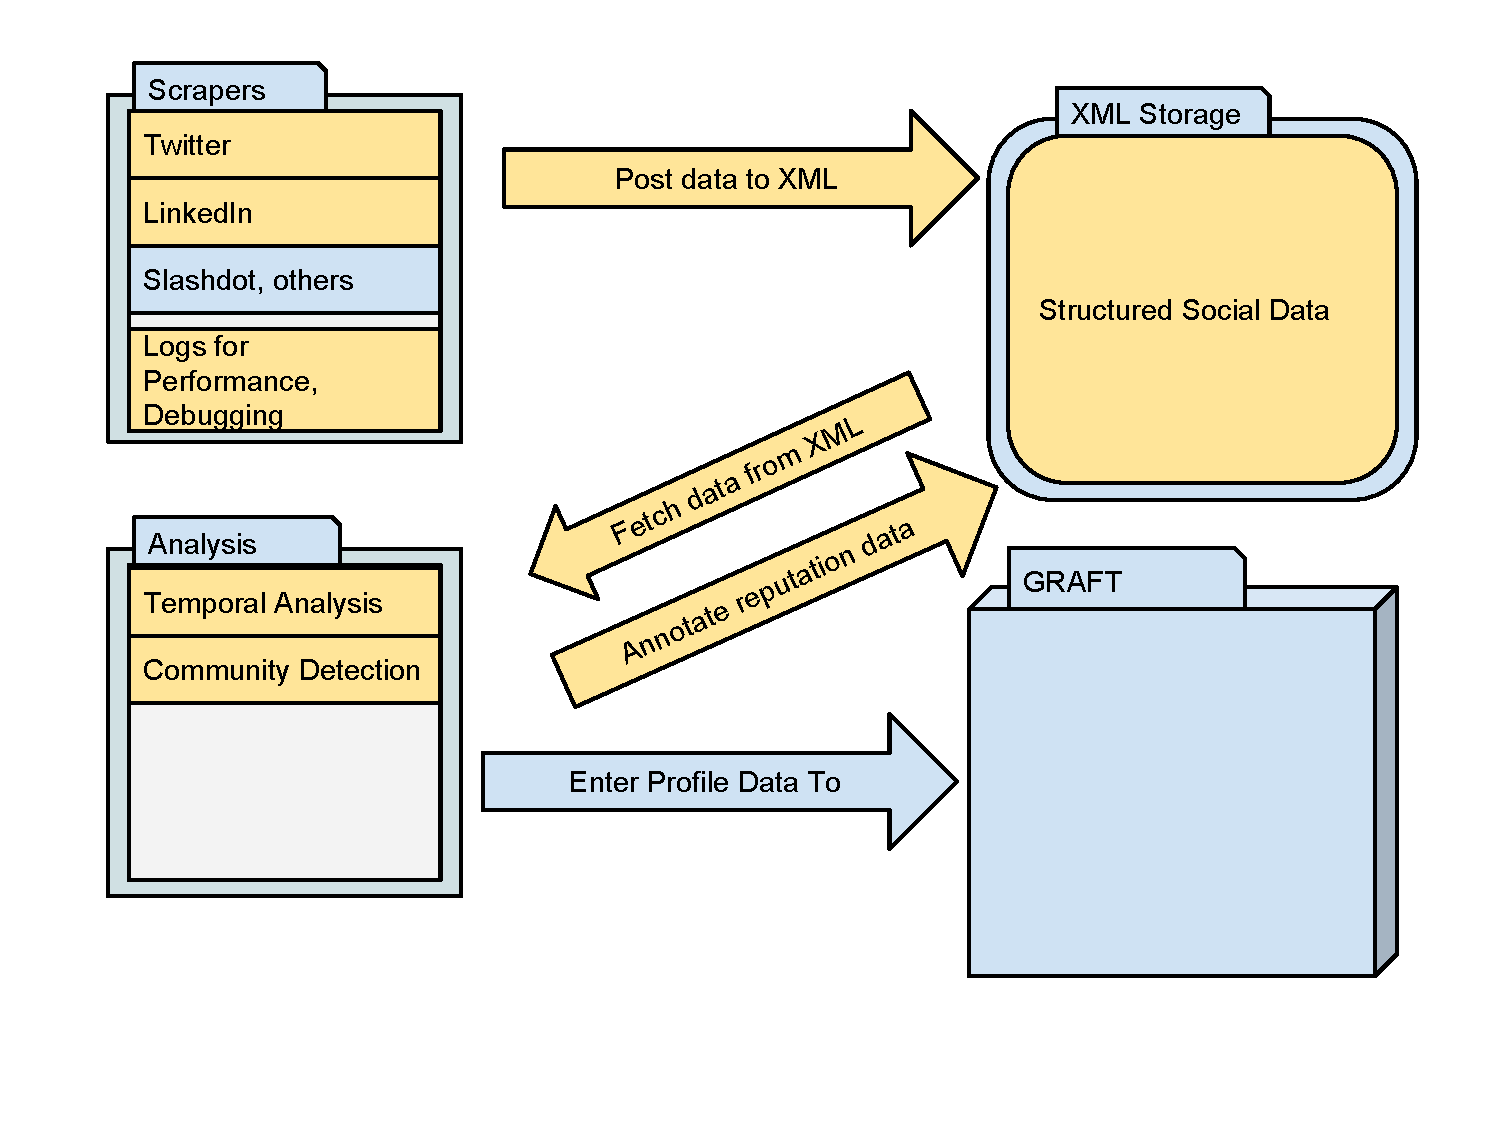
\includegraphics[width=0.7\textwidth]{Images/XML_Storage_Architecture.pdf}
\caption{Proposed Architecture for XML Storage Solution. Implemented Components are Highlighted}
\end{figure}

The advantages of this design were primarily to simplify scripting and scraper construction. Little setup was required during prototyping to construct schemas against which to save data. These prototype structures and files were simply imported into subsequent versions. An informal approach like this also allowed for straightforward manipulation of schemas, and additions to stored data. 

\section{Technology}

The web-scraper components were written entirely in Ruby. Developing screen scrapers is largely independant upon language choice; however Ruby was selected due to its large number of libraries suitable for scraping, and straightforward scripting nature. Ruby also has a significant OpenSource culture in comparison to many other languages.This was considered important early in the project when looking at developing a model for future maintenance of the scrapers, especially when considering the discarded requirement of aggregating data for GRAft. 

Alternatives to Ruby were considered; Java, which does not have the same open source following as Ruby, as well as a larger degree of lower-level network coding for web-scraping software; and PHP, which was rejected due to personal time constraints restricting personal capabilities of learning the language to a competent level during the project. PHP would have given the advantage of being more consistent with past works, however \cite{GRAft}, as well as being the same language as my policies are described in. 

The frameworks upon which my scrapers are built included:

\begin{itemize}
 \item Nokogiri: a widely used HTML and XML parsing library, allowing for straightforward interpretation of raw HTML documents.
 \item Mechanize: a library simulating browser interaction on web-pages, without requiring a real browser.
 \item Rest-Client: Ruby's most popular HTTP client.
\end{itemize}

Alternative frameworks were considered, and their advantages and reasons for not being selected in the final model will now be covered.

\subsection{Extend scrAPI}

scrAPI is a Rubyforge project, allowing for fast implementation of web scrapers. The benefit of scrAPI is that it would allow me to fetch data from HTML pages using CSS selectors. It also hid processes such as the actual fetching of pages, and sending of HTTP requests. Ultimately scrAPI was a more high-level approach to scraping content.

Extending scrAPI was ultimately discarded however, due to its heavy reliance on CSS files remaining constant. Any change to stylesheet files would likely have broken my scrapers. Arguably these stylesheets are less likely to change than layout manipulations (e.g. consider xpath on HTML as an alternative); however on sites such as Twitter and Facebook large design teams frequently make changes to these files. Given that a key requirement of the project was to make scrapers resistant to user-interface change, this resulted in scrAPI being deemed unfit for purpose. 

\subsection{Extend A Browser-Automation Model}

Browser automation options were considered as an alternative architecture. Frameworks such as Watir allow users to simulate user interaction with web pages, by driving an actual browser instance.

While this option would likely have had no issues through site detection (because of legitimate user-agents, downloading css selectors, etc), it would have been much less efficient with regards to performance. Interface changes generally result in browser-automation scripts failing, rendering this framework solution poorly maintainable in the long term. 

\subsection{Use the API}

Although the project title from the outset was 'Reputation Scraper', we investigated the use of site's APIs before settling on the scraping option. A basic application interacting with the Twitter API was constructed early in the project. Twitter's API version 1.0 was actually highly suitable for the needs of the project. However the changes in REST API v 1.1 rendered this infeasible. The earlier API allowed fetching of up to 800 statuses from any public profile, along with more public data (see appendix for more information). Version 1.1 however implemented more requirements for authentication, and limited functions such as downloading tweets to the individual's account only. Facebook's developer API is even more restricted, and in general only suitable for application developers able to obtain permissions from users. LinkedIn's policy is similar. %due to the changes!!!

\begin{figure}[h!]
\centering
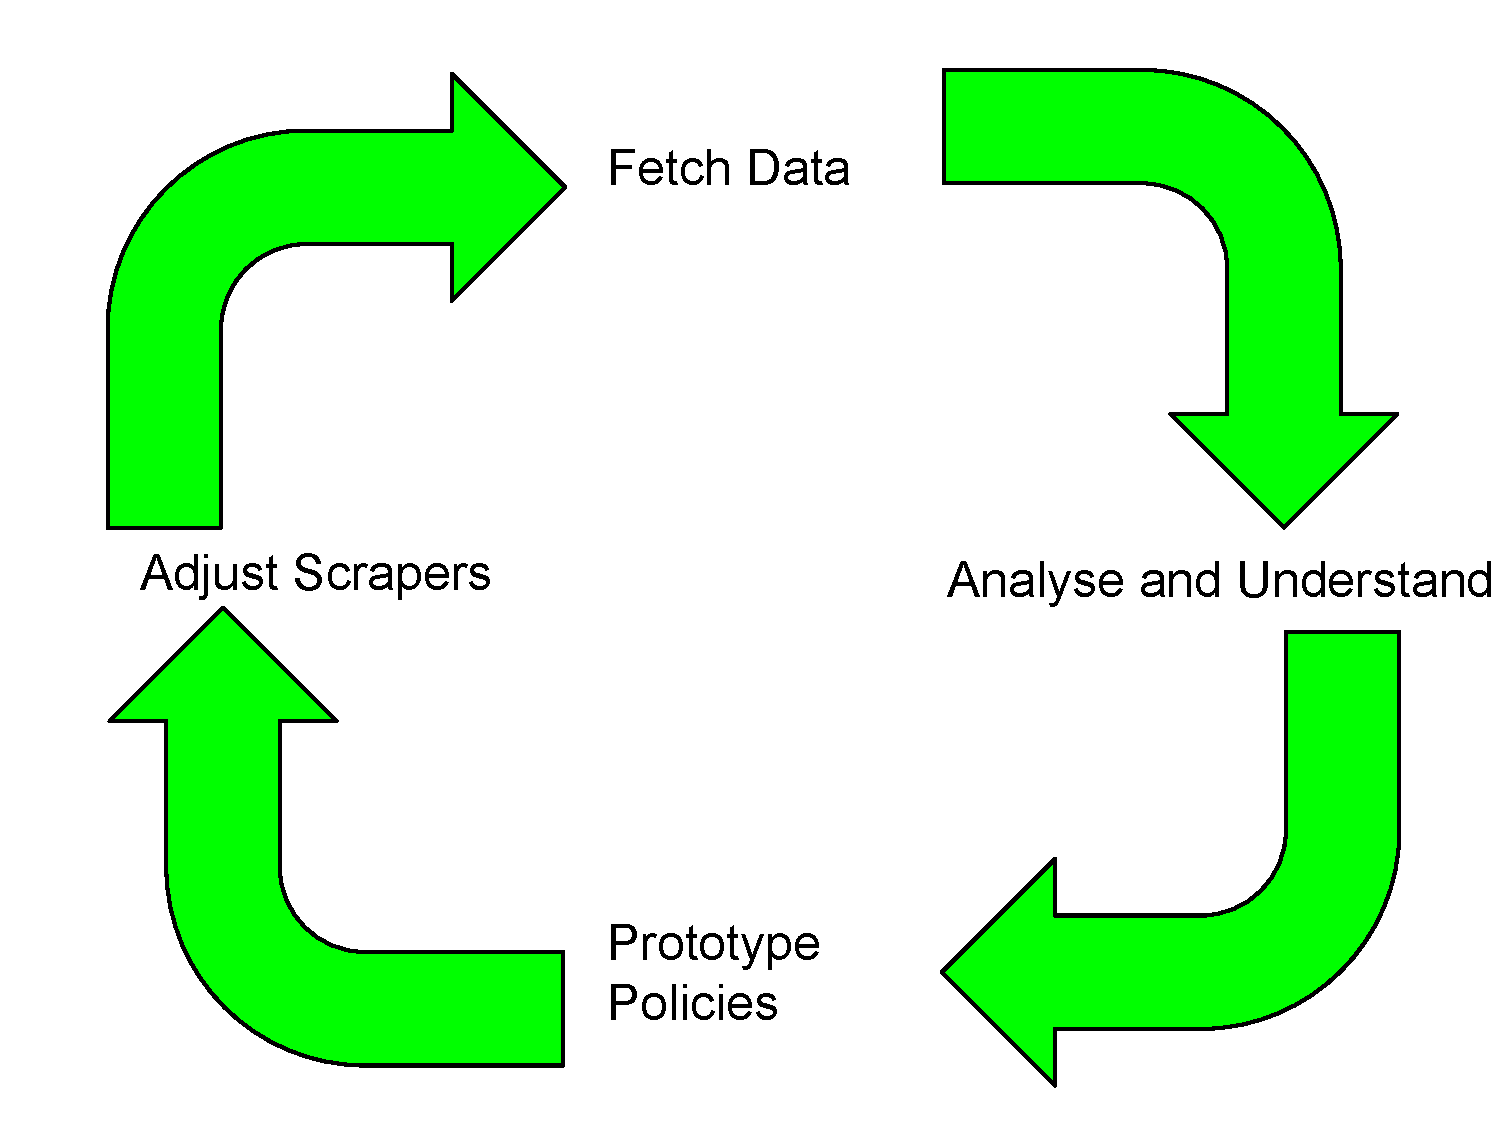
\includegraphics[width=0.3\textwidth]{Images/Implementation_Lifecycle.pdf}
\caption{Scraper Development Feedback Loop}
\end{figure}

\section{Systems Design and Structure}

Developing the project solution consisted generally of a cyclic, iterative prototyping approach as detailed in figure 5.3. This generally consisted of four phases; Implementing and adjusting scrapers, fetching data, analysing the data, and prototyping policy concepts as a result of this analysis. The first scraper developed was for Facebook. 

\section{Twitter Crawler}

The Twitter Crawler uses a Google Twitter search function, to loop through profiles at the top level. An input text file of random names delimited by lines is accepted by the scraper. These names are looped through in order, with the scraper fetching the profiles of the top 10 results returned through Google. Bias is introduced through this approach, as results appearing in Google are naturally more popular than users who would not. However as the top ten results are fetched and prepared for scraping, in general the lower ranking users here are more 'standard'. 

A potentially better approach to randomising the selection of profiles to scrape would have been to crawl through an already-generated set of random profile names. However searches did not reveal any such databases to exist, excluding 'celebrity-exclusive' ones which would have been significantly worse than my current approach. I also considered crawling via embedded links on Twitter, starting from any profile and following retweet links through to new profiles. However this introduces new complexities - how will the algorithm detect infinite loops (potentially huge loops), or detect repeat profiles? As the project was ultimately about reputation and not scraping algorithms, the simple name-searching approach was selected. 

Once the ten profile names are selected for scraping, the application will move on to the actual scraping of each of these associated 'profiles'. The definition of a Twitter profile changed throughout the project, as more information was added to be analysed. The final schema of stored data for the standard Twitter scraper is contained in appendix 1.1. Essentially all tweets are captured where possible, along with associated retweets, favourites, and the profile names of users who retweeted this item. Profile metadata is also stored, such as number of followers, number following, and total number of tweets.
%CHANGE THIS AS APPROPRIATE. 

There are a number of technical difficulties with the fetching of this data, which we will now discuss. Firstly, a twitter page does not immediately display all tweets for a user for obvious latency reasons. To view more than the initial 12 tweets, users must scroll through an infinite scrolling window which requests more data through AJAX calls. To simulate this interaction, I used chrome's 'network capture' feature to inspect requests to the page during the scrolling function. The URL is of the following form:

\begin{verbatim}
 /timeline/with_replies?include_available_features=1&include_entities=1&max_id=12345
\end{verbatim}

\noindent The JSON returned is then parsed to retrieve relevant information. As a Twitter profile may contain retweets from other profiles, checks have to also be taken at this stage to ensure the content is originally generated by the user of interest. This is as simple as checking the poster name. To increase performance I experimented with various tweet window sizes, although this was ultimately inneffective at maximising speeds for reasons covered now.

\subsection{Parallel Tweet Fetching}

Although tweet content can be fetched from the basic page, useful data such as retweet and favourite count is initially hidden. To reveal this, a further request must be sent, to view tweet detail. Fortunately, this process can be parallelised for each of the tweet windows. In the final twitter scraper a thread pool of 15 threads is created, one for each potential tweet in the window. Each thread then fetches and parses each tweet individually. To ensure parallel performance is not lost, any tweet-fetching process that fails here will simply be thrown away. Parallelisation of tweet fetching resulted in huge performance gains, which will be discussed further in chapter 6.

\subsection{Detection Avoidance}



\subsection{Dealing with Authentication}

To fetch retweet-name data, more features had to be added. All other data fetched was publicly viewable, whereas this data is only available to users who have authenticated with Twitter.

\subsection{Request Handler}

The Twitter crawler 

First implemented basic scraper components, which loop through Twitter pages.


%Mention that the code is available from github. http://www.github.com/irwalker/dat-roll

Content behind login

Infinite scrolling

Rate limiting -> encountered sometimes? 503 errors primarily

'Scraper window', not actually very effective, due to the primary networking burden being on sending a seperate HTTP request to download every tweet.

Spoofing headers -> using fake user-agents, and rotating between user agents in between overall requests.

Poorly formed markup -> was an occasional issue. Found that some libraries were more strict on this than others, and adjusted accordingly.

Authentication

Pattern scraper employed to fetch data. 

\subsection{Avoiding Detection}

The request handler component uses several strategies to avoid detection by sites. 

In order to avoid detection by websites, the request handler component of my scrapers 

%This is where I talk about the actual scraper design, and how I cope with issues like infinite scrolling etc.
%The actual code structure, and various component's roles.

\subsection{Twitter Scraper}
%How I went about implementing the Twitter scraper

Initial prototype

Design improvements, including multi-threading and parallel fetching of tweets. Decisions around discarding requests that fail in scraping individual tweets. 

\subsection{LinkedIn Scraper}

\subsection{Facebook Scraper}
%This is where I should incorporate the discussion about framework selection.


\subsection{Code instrumentation}

The code was instrumented using a Ruby logger system written for the application. Given complexities and difficulties debugging errors on web-scraping applications, logging had to be performed to a very fine level of granularity. Any action changing system state such as fetching a page triggers the logging mechanism. The logger would then take note of the timestamp and write to the appropriate file the nature of the action. For example, if the scraper sent an HTTP request to retrieve a given URL, it would record the timestamp and URL requested. 

The logger would write to the appropriate log file based on the nature of the supplied action. Because these scrapers were running over long periods of time, using traditional IDE debugging tools was not effective at detecting errors. As a result, I used multiple debugging files with different purposes in an attempt to catch these errors. The debug.log captured all interaction information at a basic level. Error.log captures error information that is non-fatal to scraping an individual's profile, e.g. on Twitter. Commonly these errors were due to application logic flaws, such as performing operations on null entities. As a result the error.log assisted greatly in identifying these edge cases. Finally the failure.log was used to record fatal exceptions that would prevent me from scraping a profile. Occurences such as 404, 500 or 503 responses from servers are examples that would result in a record being written to the failure log. The failure log would write system state at the time of failure to a high level 
of detail, sometimes even writing the entire HTML document before the failure to disk. This again assisted with debugging, when reviewing how a particular run had gone. 

To limit the performance overhead of writing to these logging files, a buffered approach was taken in order to achieve the least impact. %lol
